\documentclass[12pt]{ctexart}

\usepackage{graphicx}
\usepackage[hmargin=1.1in,vmargin=1in]{geometry}
\usepackage{indentfirst}
\usepackage{multirow}
\usepackage{makecell}
\usepackage{amsmath}
\usepackage{amssymb}
\usepackage{gbt7714}
\usepackage[defaultmono,scale=0.85]{droidsansmono}
\usepackage[colorlinks=true]{hyperref}

\bibliographystyle{gbt7714-numerical}

\fontsize{14pt}{1.0}

\newlength{\blanklength}
\setlength{\blanklength}{40ex}

\providecommand{\thetitle}{LPBoost 相关论文阅读报告}
\providecommand{\theauthor}{Sparky\_14145}
\providecommand{\thestudentID}{71XXXXXX}
\providecommand{\theemail}{Sparky\_14145@outlook.com}
\providecommand{\theinstitution}{College of Software Engineering}

% \input{personal_info/info.tex}

\providecommand{\blankToFill}[1]{
    \parbox[t][3ex]{\blanklength}{
        \makebox[\blanklength]{#1}\\[0pt]
        \rule[2ex]{\blanklength}{0.1ex}
    }
}

\providecommand{\makecover}{\begin{titlepage}
    \noindent
    {东南大学} \\[2pt]
    {\Large \bfseries 课程报告}

    \vspace*{20pt}
    \begin{center}
    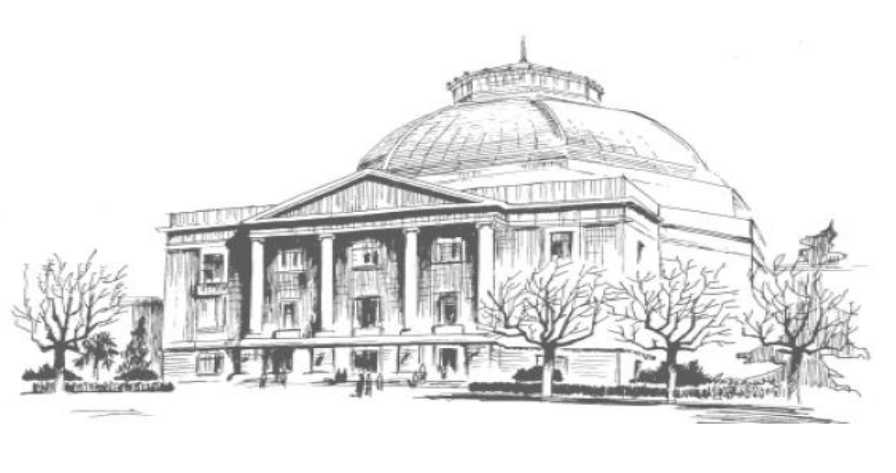
\includegraphics[width=0.8\textwidth]{pics/cover.png} \\
        \textsc{\Huge 机器学习} \\[2pt]
        \textsc{\huge 课程报告}

        \vspace*{10pt}
        \begin{tabular}[c]{rc}
            题目        & \blankToFill{\thetitle} \\
            日期        & \blankToFill{\today} \\
            姓名        & \blankToFill{\theauthor\footnotemark} \\
            学号        & \blankToFill{\thestudentID} \\
            学院        & \blankToFill{\theinstitution} 
        \end{tabular}
        \rmfamily
    \end{center}

    \vspace*{0pt}
    \footnotetext{\theemail}
\end{titlepage}}

\begin{document}
    \makecover

    \section{背景}

    利用许多弱分类器(这些分类器可能只比一个完全随机的分类器要稍微``好''一点点),来生成一个强分类器,这就是集成学习中的 Boosting 算法。要实现将弱分类器转换成强分类器有很多种方法,最直观的想法是能不能仅仅通过简单的线性组合,将所有的弱分类器的输出按照某一权重比例直接相加,来得到一个强分类器,同时以这个分类器的最小边界作为目标函数并以此来判定得到的强分类器的好坏。

    \section{介绍}

    将以上想法中的``某一权重''用线性规划求出来,并尝试最大化最小边界,这就是 LPBoost(Linear Programming Boosting)。

    具体来说,LPBoost 是一种有监督集成学习算法,通过线性组合一系列的弱分类器 $h(\pmb{x})$,得到一个强分类器 $f(\pmb{x})$,并用线性规划来找到一个组合方案,使得在这个方案下,整个数据集的最小边界值最大。

    LPBoost 的一种线性规划问题如下:

    \begin{align*}
        \min_{\pmb{a}, \pmb{\xi}} & \sum_{i=1}^m a_i + C \sum_{i=1}^l \xi_i & \\
        \text{s.t.} & y_i \sum_{j=1}^m a_j h_j(\pmb{x_i}) & i = 1,\ldots,l \\
         & a_i \geq 0, i = 1,\ldots,m &
    \end{align*}

    其中:$\pmb{a}_{m \times 1}$ 是各个弱分类器的系数向量,$\pmb{\xi}_{l \times 1}$ 是松弛变量,$C$ 是惩罚系数,$l$ 是样本集容量,$m$ 是分类器个数,$(\pmb{x_i}, y_i) \in \chi \times \{-1, +1\}$ 是各个样本。它的对偶问题如下:

    \begin{align*}
        \max_u & \sum_{i=1}^l u_i & & \\
        \text{s.t.} & \sum_{i=1}^l u_iy_ih_j(\pmb{x}_i), & j &= 1,\ldots,m \\
         & 0 \leq u_i \leq C, & i &= 1,\ldots,l
    \end{align*}

    而它的另外一种被称为 $\nu$-LP Boosting 的形式如下:

    \begin{align*}
        \max_{\pmb{a,\xi},\rho} & \rho - D \sum_{i=1}^l \xi_i & & \\
        \text{s.t.} & y_i \sum_{j=1}^m a_j h_j(\pmb{x_i}) + \xi_i \geq \rho, & i &= 1,\ldots,l \\
         & \sum_{i=1}^m a_i = 1, \xi_i \geq 0, & i &= 1,\ldots,l \\ 
         & a_j \geq 0, & j &= 1,\ldots,m
    \end{align*}

    它的对偶问题:

    \begin{align*}
        \min_{\pmb{u},\beta} & \beta & & \\
        \text{s.t.} & \sum_{i=1}^l u_i y_i h_j(\pmb{x_i}) \leq \beta, & j &= 1,\ldots,m \\
         & \sum_{i=1}^l u_i = 1, 0 \leq u_i \leq D, & i &= 1,\ldots,l
    \end{align*}

    在给定的参数 $C$ 与 $D$ 满足一定条件,那么两种形式的线性规划问题是等价的。确切来说,如果原始形式的问题有原始解 $(\pmb{\overline{a}}, \overline{\rho} > 0, \pmb{\overline{\xi}})$ 与对偶解 $(\pmb{\overline{u}}, \overline{\beta})$,那么对应的 $\nu$-LP Boosting 形式的原始解与对偶解分别为 $(\pmb{\widehat{a}} = \frac{\pmb{\overline{a}}}{\overline{\rho}}, \pmb{\widehat{\xi}} = \frac{\pmb{\overline{\xi}}}{\overline{\rho}})$ 与 $(\pmb{\widehat{u}} = \frac{\pmb{\overline{u}}}{\overline{\beta}})$,且参数 $C = \frac{D}{\overline{\beta}}$。

    此外,如果在实践中选择 $D = \frac{1}{l\nu}$,其中 $\nu \in (\frac{1}{n}, 1)$ 为另一参数,那么这个新参数 $\nu$ 还会有一些特殊的性质:

    \begin{enumerate}
        \item $\nu$ 是训练集分类错误比例的上界,即设 $k$ 表示分类错误的样本,则 $\frac{k}{l} \leq \nu$;
        \item $\nu$ 是分类边界上或边界外的训练样本比例的下界;
        \item 如果那么最优解所对应的权重向量 $\pmb{a}$ 将会很稀疏,即只有一小部分弱分类器实际参与分类工作;且得到的模型只依赖训练样本中较小的子集。
    \end{enumerate}

\end{document}